\section{Formal Definition of PASS Process Models in OWL}
\label{sec:formalModelStrucutreOWL}

As mentioned in previous sections, the formal specification for the structure of the Parallel Activity Specification Schema process modeling language exists as an ontology formulated in the Web Ontology Language (OWL). This ontology is called the \textbf{Standard\_PASS\_Ont} and currently hosted at: 
\url{https://github.com/I2PM/Standard-Documents-for-Subject-Orientation/blob/master/PASS-OWL/standard_PASS\_ont\_v\_1.0.0.owl}.

In OWL there four principle concepts and color coded as shown here: \textcolor{OWLclass}{\textbf{Classes}}, relationships between classes, the so-called \textcolor{OWLObjectProperty}{\textbf{Object Properties}}, non-linking  \textcolor{OWLDataAttribute}{\textbf{Data Properties}} that are attached to classes and allow attaching individual data values to instances of the classes, and finally the instances of classes themselves, the OWL \textcolor{OWLIndividual}{\textbf{Individuals}}.



\subsection{Application Concept of the Standard PASS Ontology}

The usage of OWL as the technology for the specification comes with an intended concept of how the Standard PASS Ontology is supposed to be used as the technical foundation for an model exchange standard, next to its being a formal definition of PASS on a conceptual level.

In principle, the structure of PASS is defined with  \textcolor{OWLclass}{\textbf{Classes}},  \textcolor{OWLObjectProperty}{\textbf{Object Properties}}, and   \textcolor{OWLDataAttribute}{\textbf{Data Properties}} in the Standard PASS Ont. The actual PASS process models consist of OWL \textcolor{OWLIndividual}{\textbf{Individuals}} that adhering to the classes and rules defined in the Standard PASS ont, but will be saved in their own individual OWL Files or equivalent OWL/RDF storing systems.

The following Figures \ref{fig:ontAndModel} and \ref{fig:ImportOnt} taken from \cite{elster:ont} describes the application concept for how a process model should be saved in an individual model ontology file while referring to the standard definition ontology. At the same time, an according model may refer to other ontological specifications that contain additional but logically consistent and compatible, extensions to the standard.

%\begin{figure}[ht]
%	\centering
%	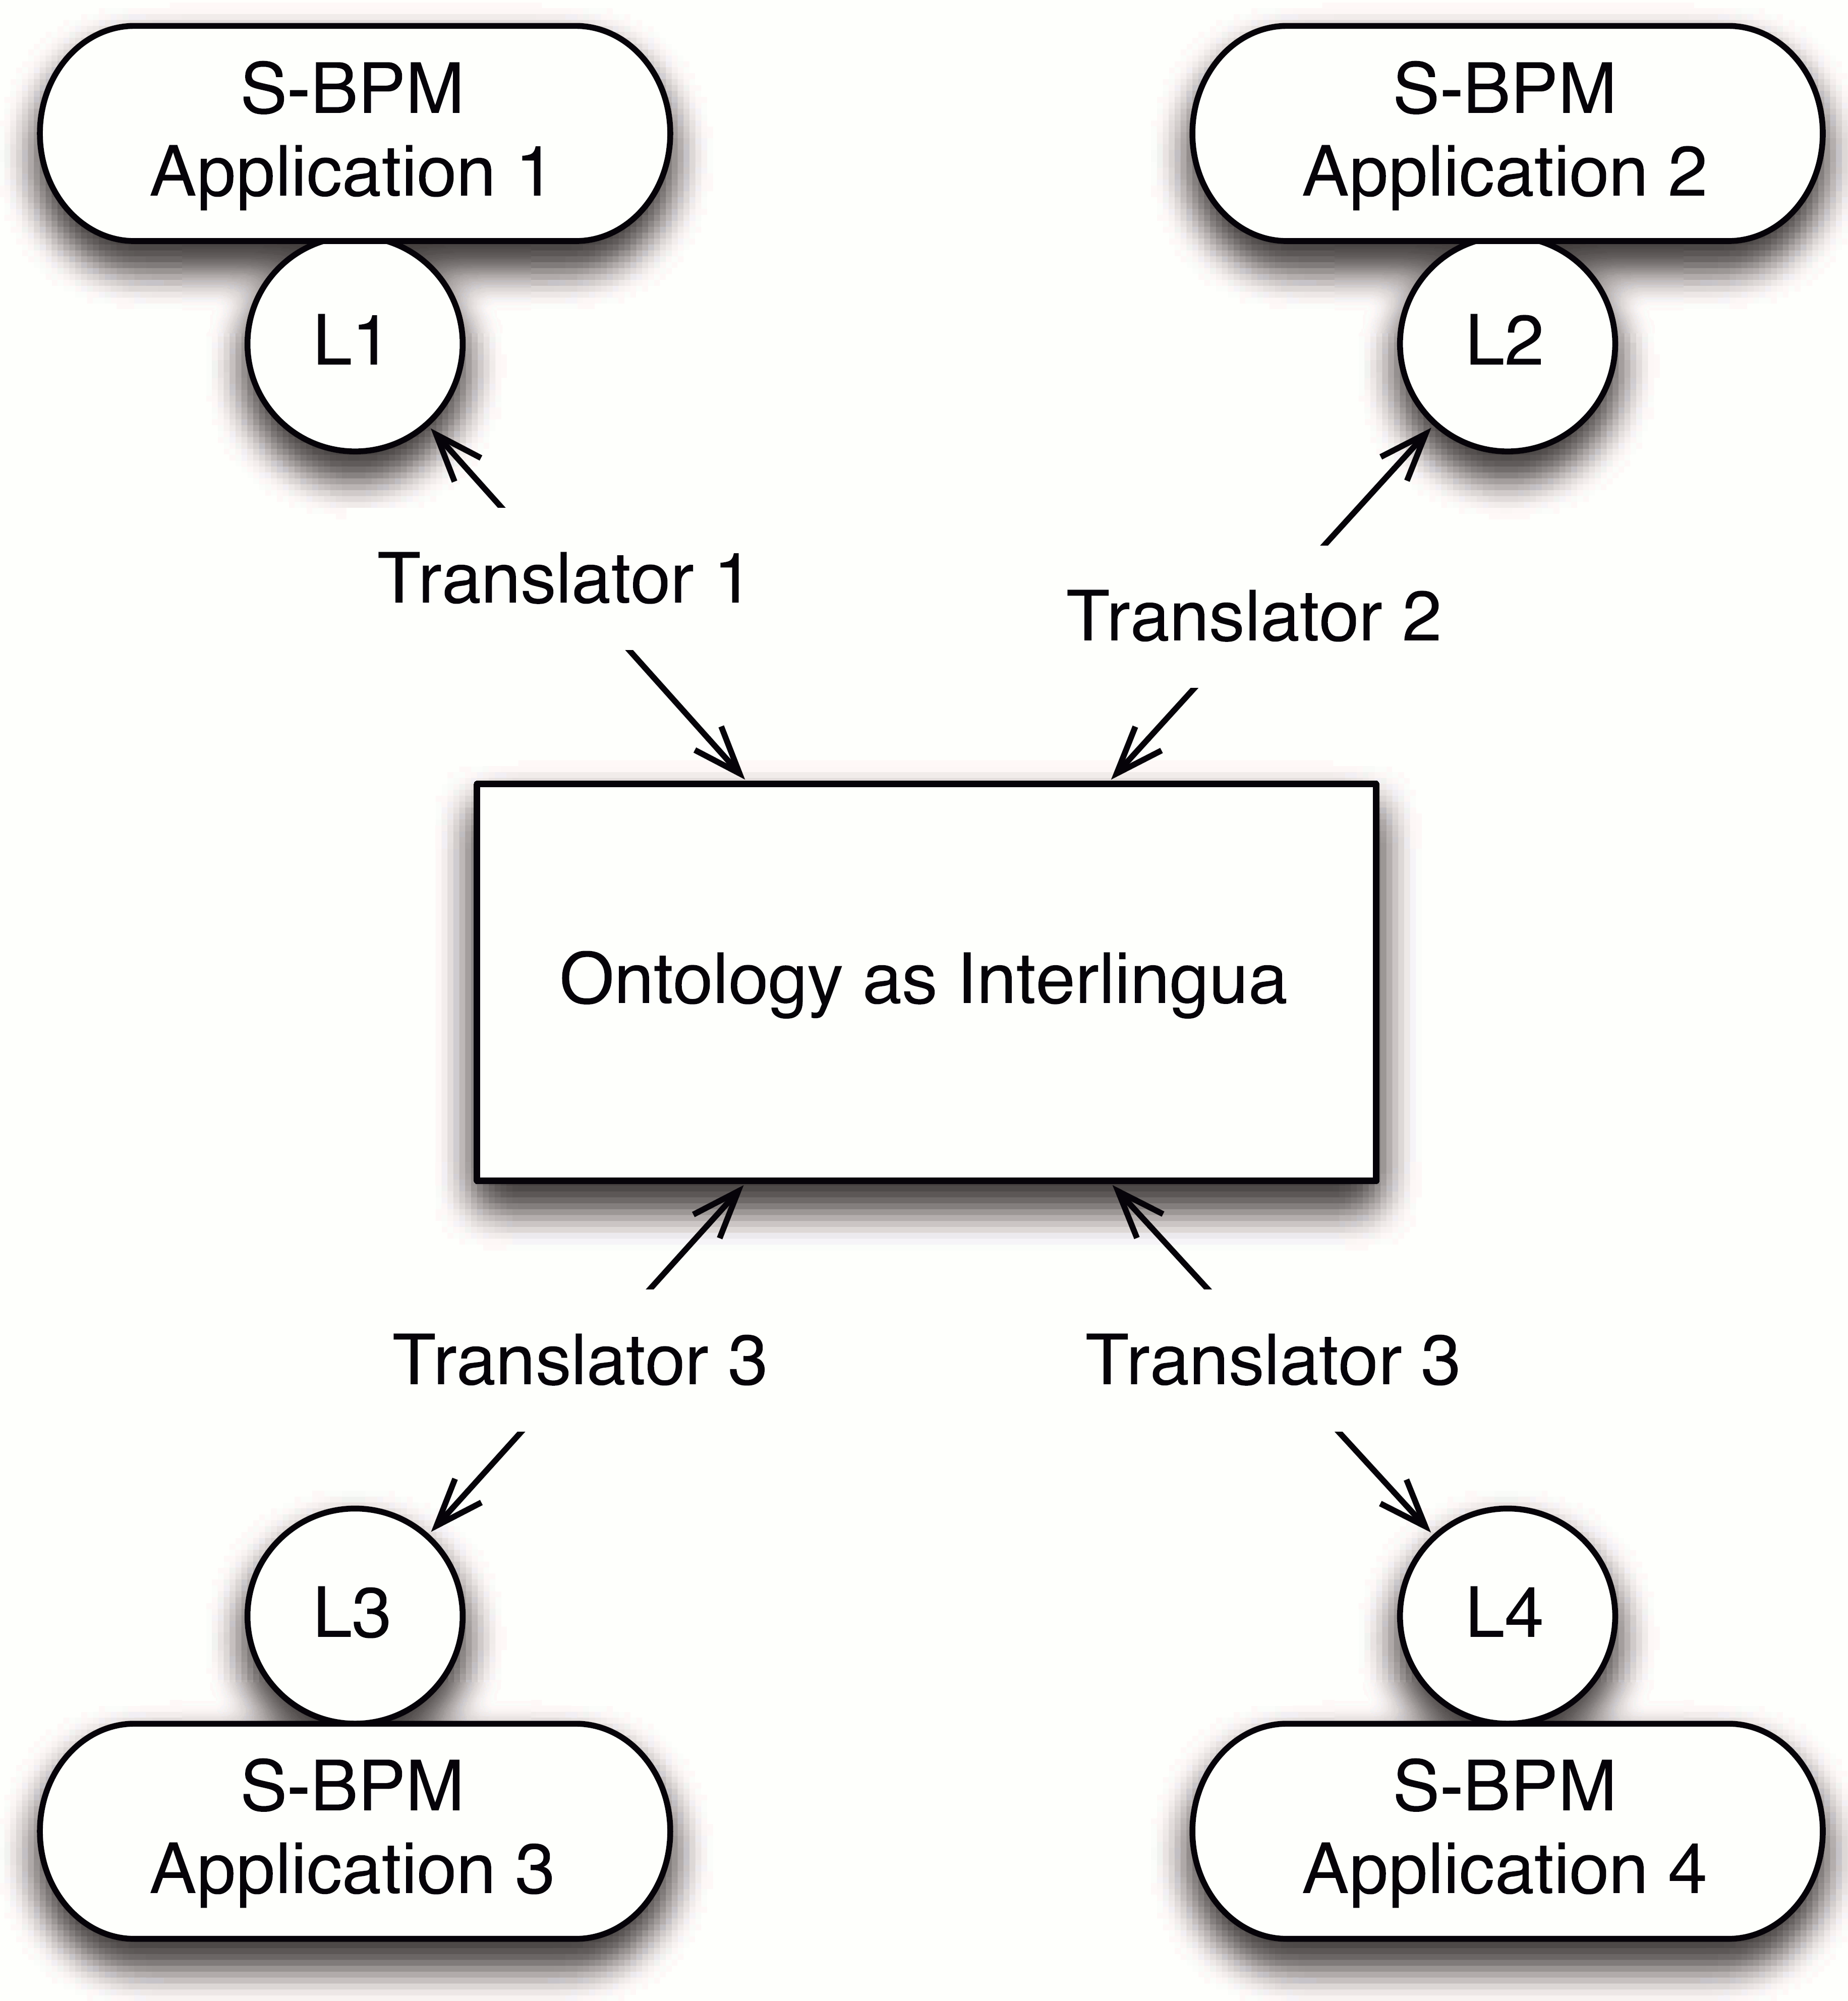
\includegraphics[width=0.50\textwidth]{Figures/Ontology/Introduction/hoeverproposal.png}
%	\caption{Ontology as interchange format proposed by g\cite{Hoever:ont}}
%\end{figure}

\begin{figure}[ht]
	\centering
	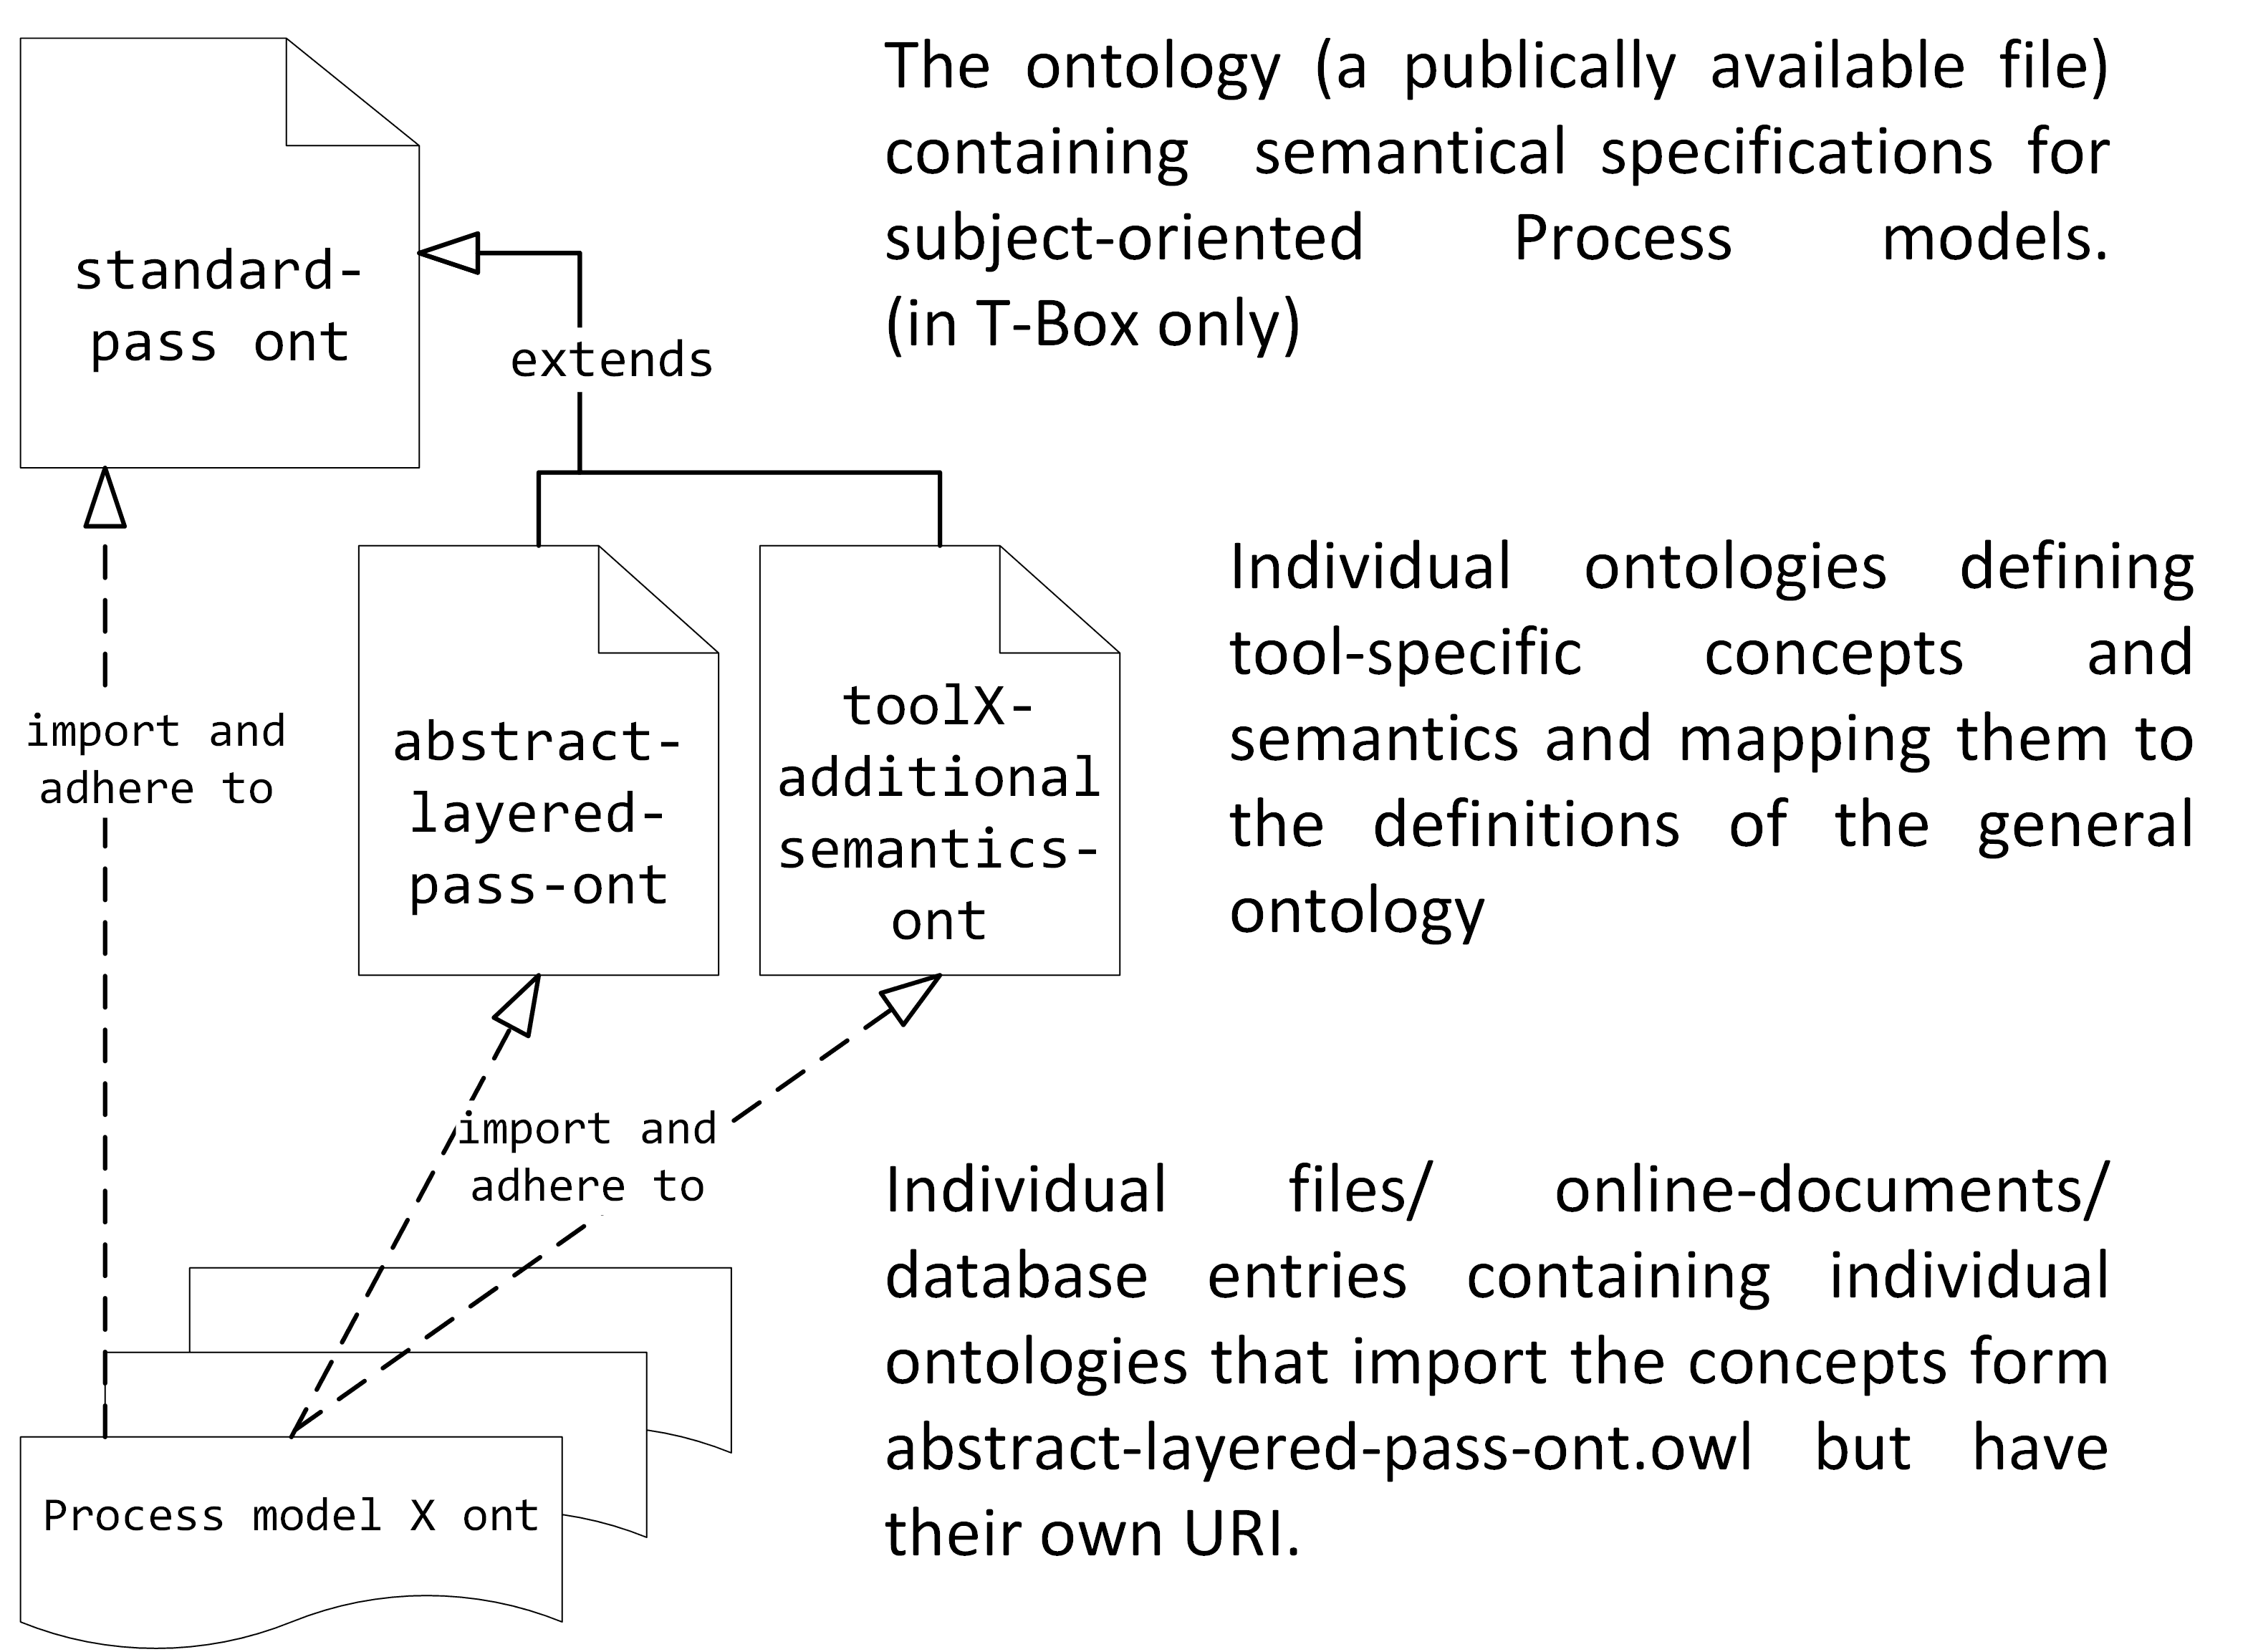
\includegraphics[width=0.7\textwidth]{Figures/Ontology/Introduction/ont-and-models.png}
	\caption{Proposed use and interaction of ontologies (from \cite{elster:ont} ).}
	\label{fig:ontAndModel}
\end{figure}

\begin{figure}[ht]
	\centering
	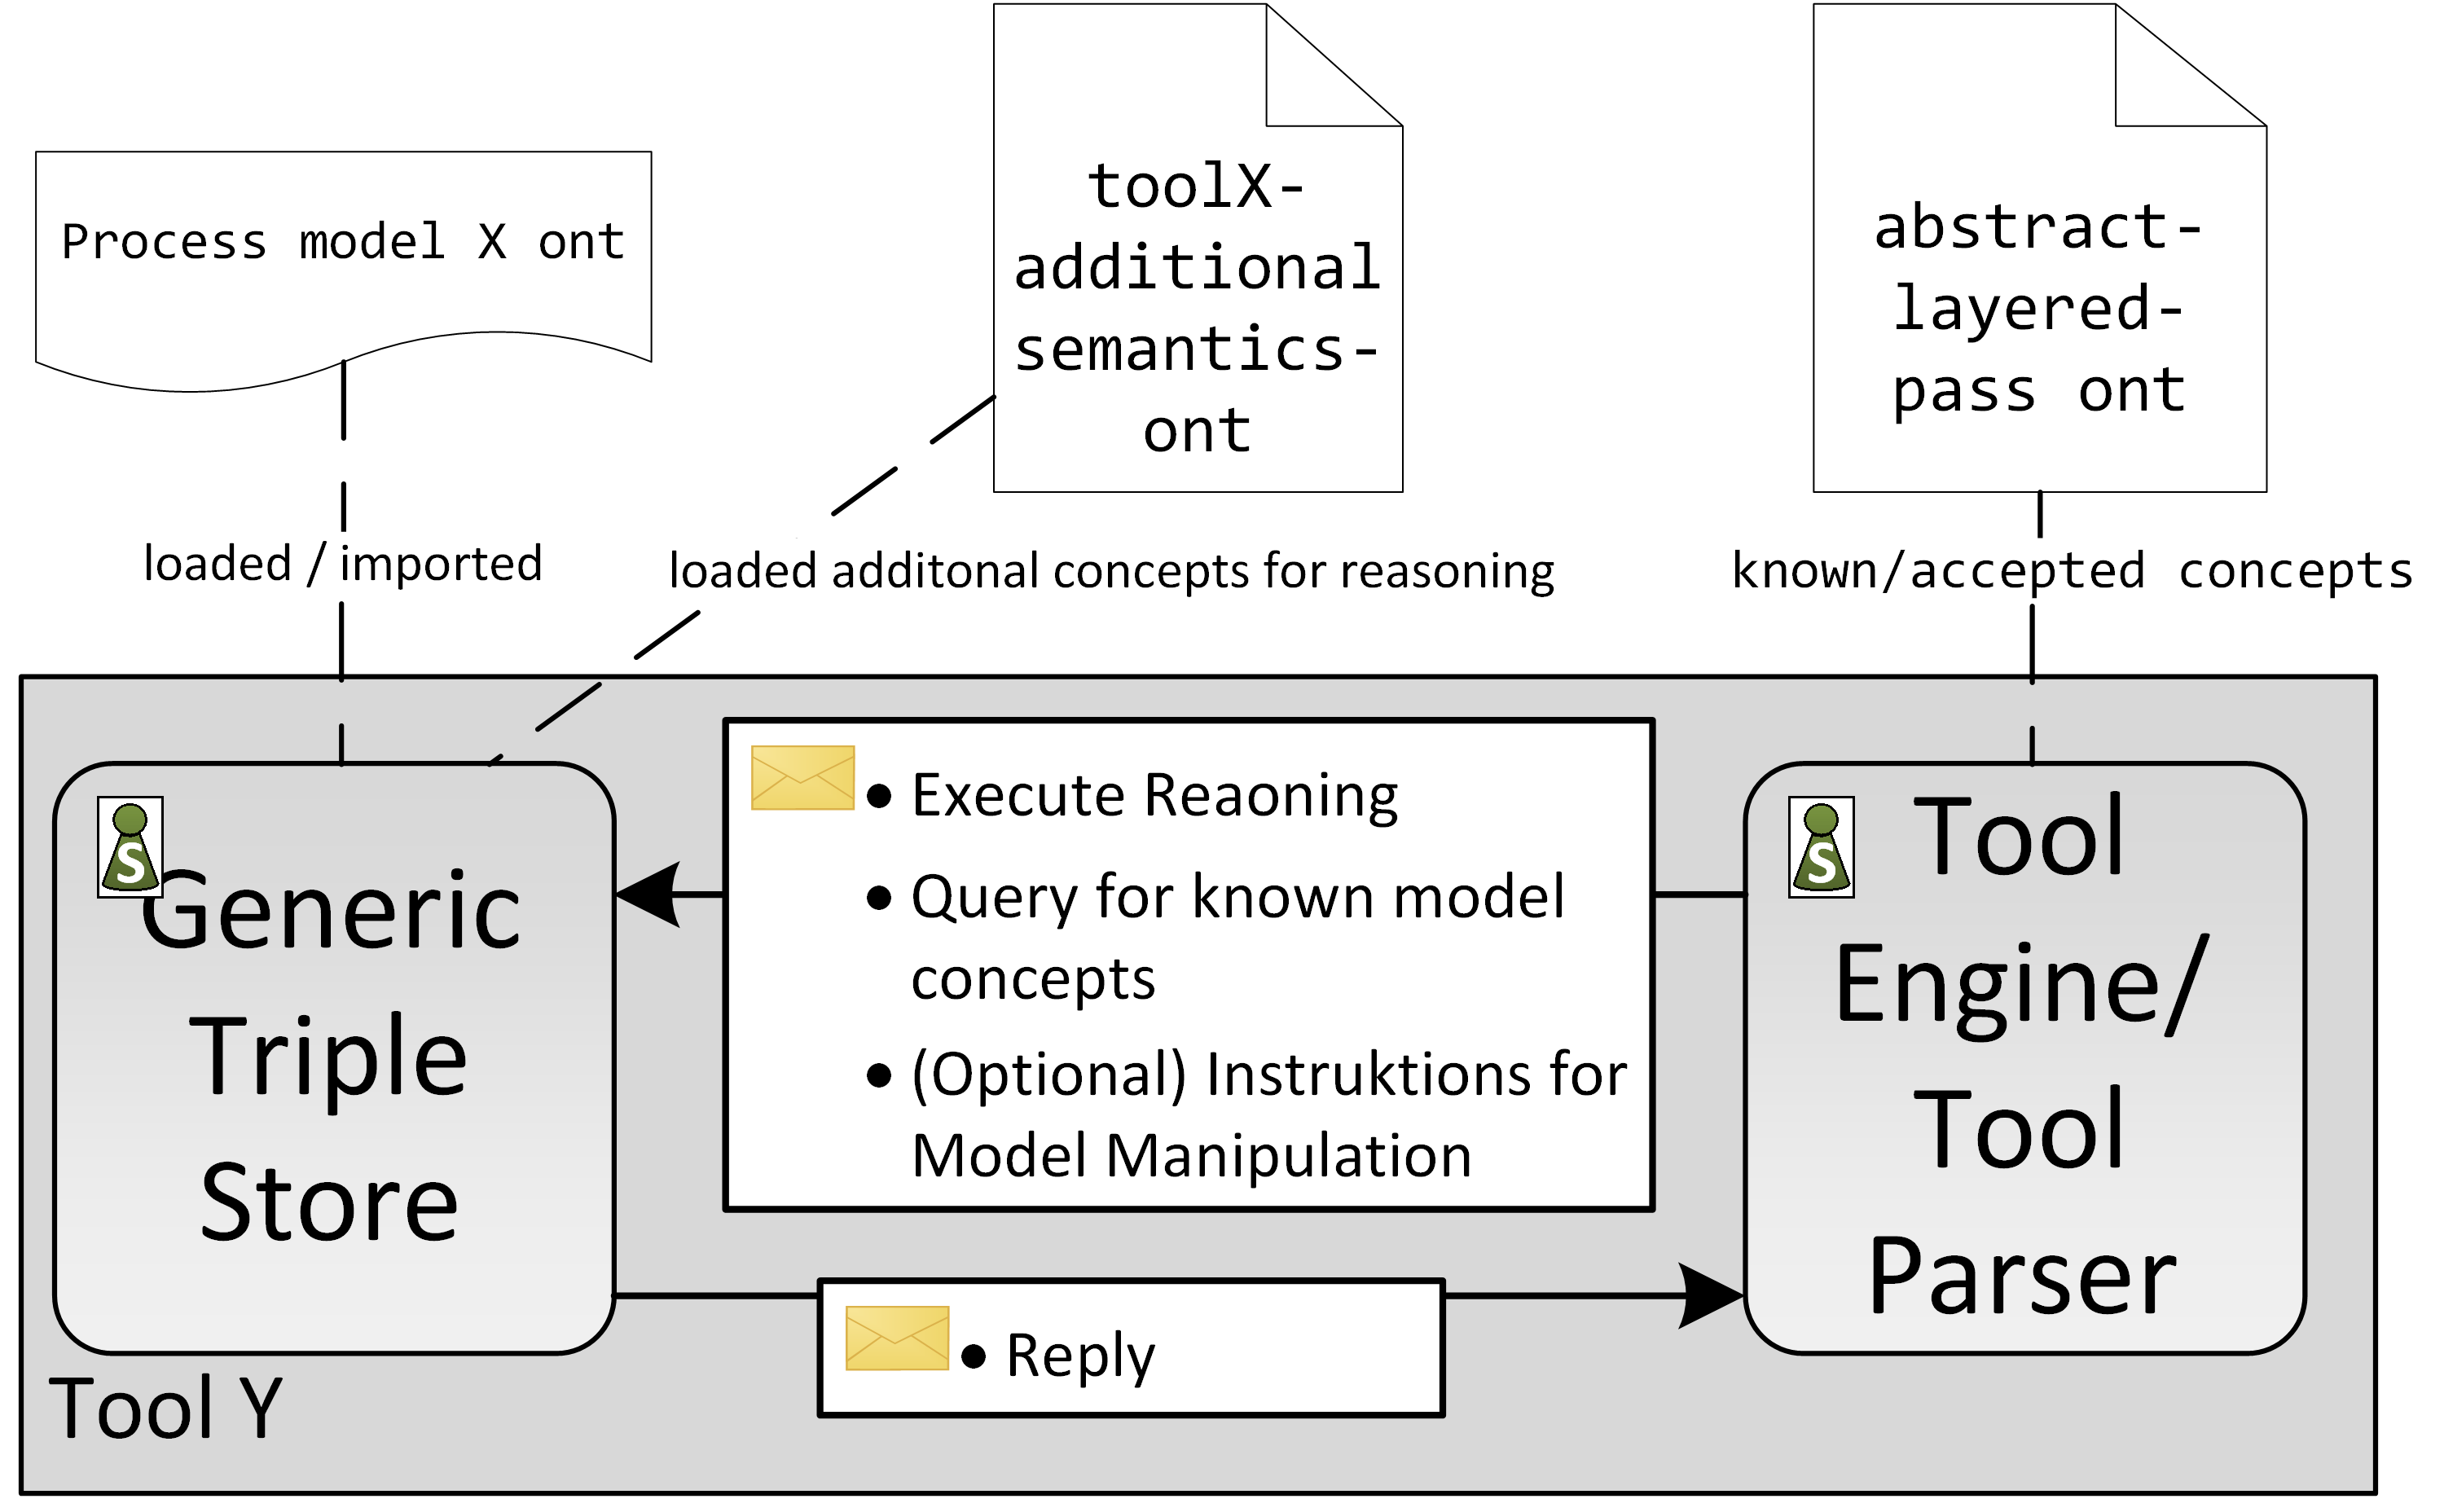
\includegraphics[width=0.50\textwidth]{Figures/Ontology/Introduction/importWorkflow.png}
	\caption{Conceptual Import Process (SID) (from \cite{elster:ont}). }
	\label{fig:ImportOnt}
\end{figure}


%\underline{\textit{\textbf{Übergang von informeller zur formalen Beschreibung sehr abrupt und unverstaändlich}}}

\subsection{ The Principle Structure of PASS in the Standard}

As a formal specification document, the Standard PASS Ont currently is comprised of roughly 4000 lines of XML/RDF/OWL code\footnote{This may differ in other OWL encoding styles such as Turtle script}. Ideally, it should be perceived using a specialized ontology/OWL editor such as e.g. the open source tool Protegée. 

Listing the entire content and detail of the specification here in written form is not useful; introducing the general structure as orientation, however is. 

The following figure \ref{fig:20171217-passprocessmodellelement} gives an overview of the general structure of the PASS OWL specifications. 


\begin{figure*}[htbp]
	\centering
	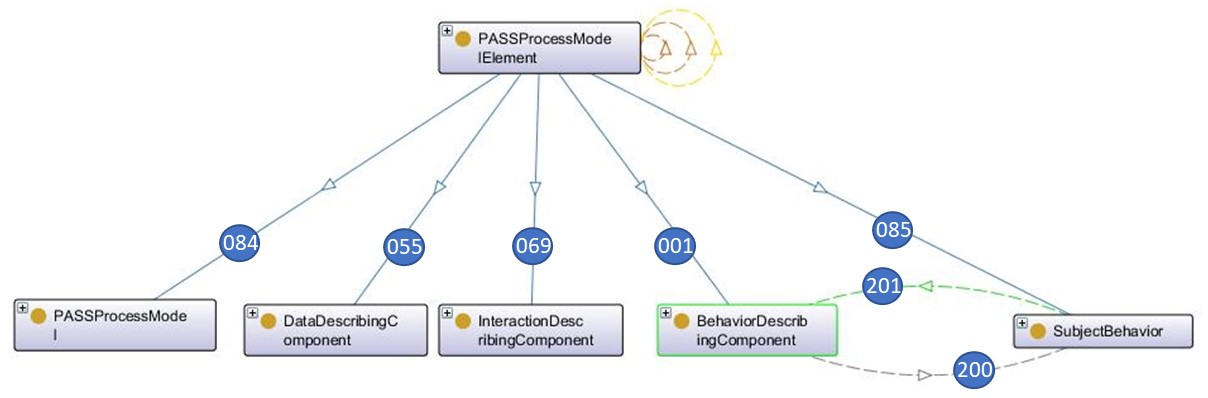
\includegraphics[width=0.9\linewidth]{Figures/Ontology/SubjectInteraction/20171217-PASSProcessModellElement}
	\caption[Elements of PASS Process Models]{Elements of PASS Process Models}
	\label{fig:20171217-passprocessmodellelement}
\end{figure*}

All elements of a PASS model are instances of sub classes of the general super-class \PASSModelElement{PASSProcessModelElement}.
\PASSModelElement{PASSProcessModelElement} has five sub-classes (subclass relations 084, 055, 069, 001 and 085 in figure \ref{fig:20171217-passprocessmodellelement}) that together form PASS process Descriptions. Instances of the classes \PASSModelElement{PASSProcessModel}, \PASSModelElement{DataDescriptionComponent}, \PASSModelElement{InteractionDescribingComponent} are used for defining the structural aspects of a process specification in PASS. The classes \PASSModelElement{SubjectBehavior} and its content element the \PASSModelElement{BehaviorDescribingComponent}  define the dynamic aspects, namely in which sequences messages are sent and received or internal actions are executed.

\subsection{PASS Process Model Elements and PASS Process Model}

Any \PASSModelElement{PASSProcessModelElement}, including the  \PASSModelElement{PASSProcessModell} itself has at least one name (\PASSModelElementObjectPropertie{hasModelComponentLabel}) and exactly one individual ID (\PASSModelElementObjectPropertie{hasModelComponentID})\footnote{When OWL technology is employed the ID of a model element ideally coincides with its URI or parts of it. However, not necessarily}.Any model element also can be equipped with \PASSModelElement{Additional Attributes} (\PASSModelElementObjectPropertie{hasAdditionalAttribute} - property 208 in \ref{fig:20171217-passprocessmodellelement}). 

The central entities of a PASS process model are subjects which represent the active elements of a process and the messages they exchange. Messages transport data from one subject to others (payload). Figure \ref{fig:20181217-passprocessmodel} shows the corresponding ontology for the PASS process models.

\begin{figure*}[htbp]
	\centering
	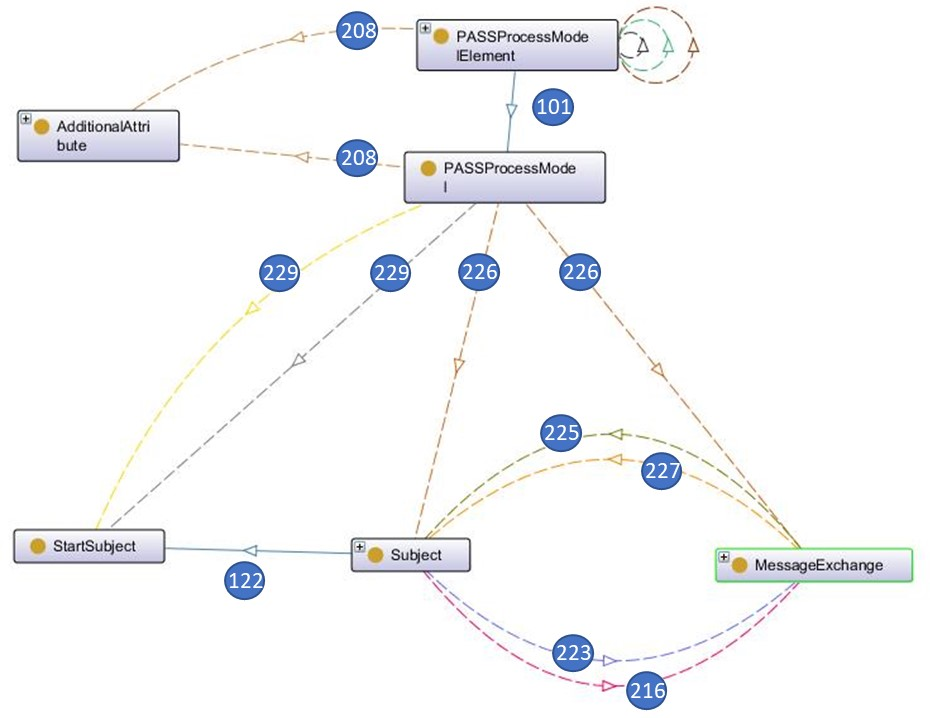
\includegraphics[width=1.0\linewidth]{Figures/Ontology/SubjectInteraction/20181217-PASSProcessModel}
	\caption[PASS Process Modell]{PASS Process Modell}
	\label{fig:20181217-passprocessmodel}
\end{figure*}


The class \PASSModelElement{Subject} and the class \PASSModelElement{MessageExchange} have the general relation (\PASSModelElementObjectPropertie{hasRelation}) to any other \texttt{model elements} as well as the class \PASSModelElement{PASSProcessModel} (property 226 in \ref{fig:20171217-passprocessmodellelement}). 

The properties \PASSModelElementObjectPropertie{hasReceiver} and \PASSModelElementObjectPropertie{hasSender} express that a Message Exchange has a sending and receiving subject (properties 225 and 227 in \ref{fig:20171217-passprocessmodellelement}) whereas the according inverse properties \PASSModelElementObjectPropertie{hasOutgoingMessageExchange} and \PASSModelElementObjectPropertie{hasIncomingMessageExchange} define which messages are sent or received by a subject. The property \PASSModelElementObjectPropertie{hasStartSubject} (property 229 in \ref{fig:20171217-passprocessmodellelement}) defines a start subject for a \PASSModelElement{PASSProcessModell}. A start subject is a subclass of the class subject (subclass relation 122 in \ref{fig:20171217-passprocessmodellelement}).

\subsection{Interaction Describing Components}

The following figure \ref{fig:ontogrsubjectinteraction} shows the subset of the classes and properties required for describing the interaction of subjects, the \PASSModelElement{Interaction Describing Components}.

\begin{figure*}[htbp]
	\centering
	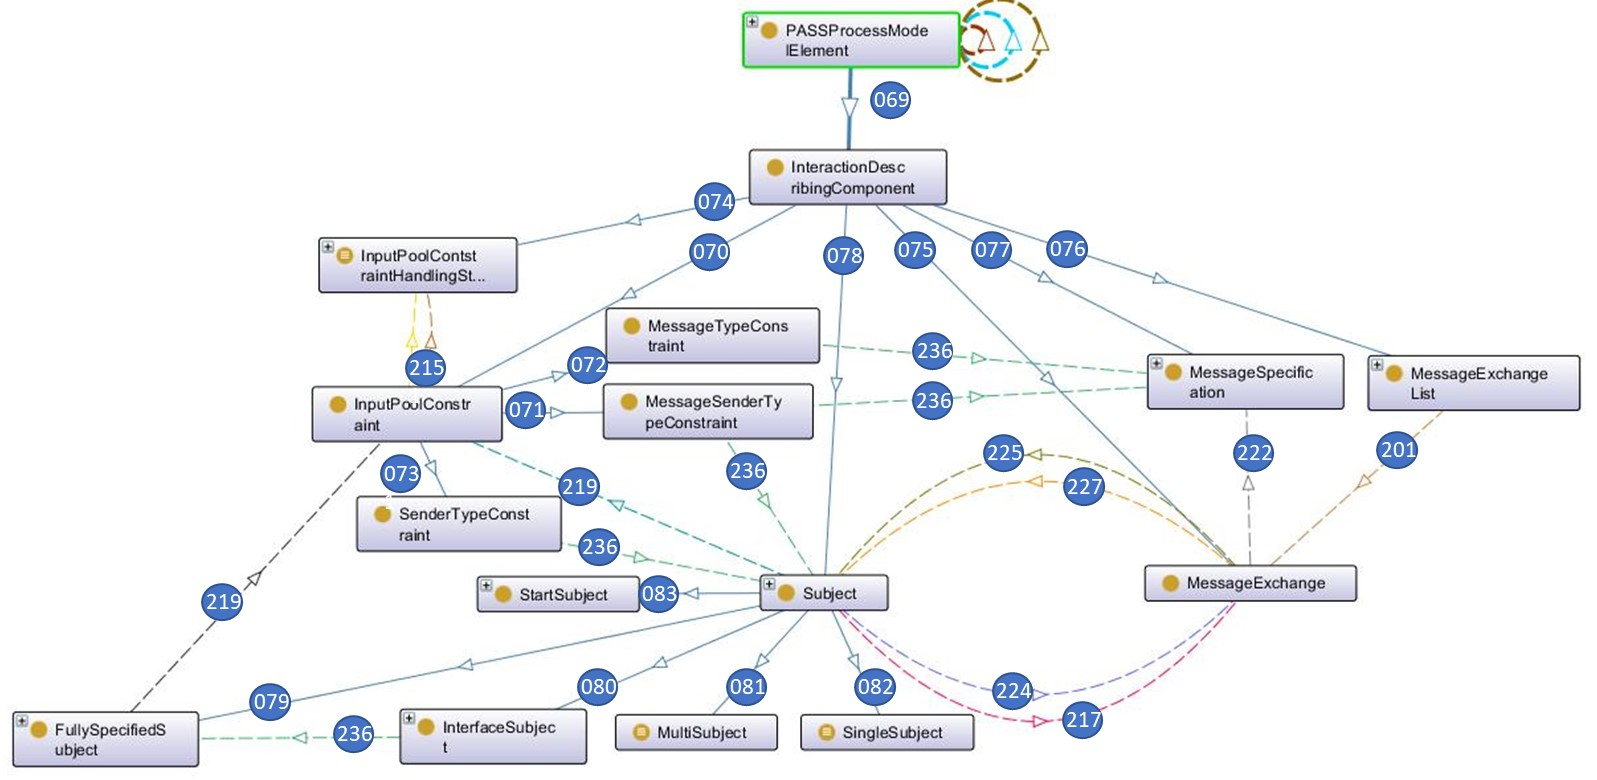
\includegraphics[width=1.0\linewidth]{Figures/Ontology/SubjectInteraction/OntoGrSubjectInteraction}
	\caption[Subject Interaction Diagram]{Subject Interaction Diagram}
	\label{fig:ontogrsubjectinteraction}
\end{figure*}

The central classes are \PASSModelElement{Subject}, \PASSModelElement{MessageSpecification}, and \PASSModelElement{MessageExchange}. Between these classes are defined the properties  \PASSModelElementObjectPropertie{hasIncomingMessageExchange} (in figure \ref{fig:ontogrsubjectinteraction} number 217) and  \PASSModelElementObjectPropertie{hasOutgoingMessageExchange} (in figure \ref{fig:ontogrsubjectinteraction} number 224). These properties define that subjects have incoming and outgoing messages. Each \PASSModelElement{MessageExchange} has a sender and a receiver (in figure \ref{fig:ontogrsubjectinteraction} number 227 and number 225). Messages Exchanges also have a type. This is expressed by the property \PASSModelElementObjectPropertie{hasMessageType} (in figure \ref{fig:ontogrsubjectinteraction} number 222) linking it to a \PASSModelElement{MessageSpecification}. These Message Specifications are the actual existential definitions for Messages, while the model element of the Message Exchange are used to define that an existing message is indeed exchanged between specific subjects. Beyond that, message exchanges that have the same sender and receiver may be grouped into an \PASSModelElement{MessageExchangeList} that \PASSModelElementObjectPropertie{contains} them.

During execution, each Subject has an Input Pool. Input pools can be restricted by three types of constraints (see section \ref{sec:inputpool}). This is expressed by the according property references  (in figure \ref{fig:ontogrsubjectinteraction} number 236) and \PASSModelElement{InputPoolConstraints} (in figure \ref{fig:ontogrsubjectinteraction} number 219). Constraints which are related to certain messages have references to the class \PASSModelElement{MessageSpecification}.

There are four sub-classes of the class \PASSModelElement{Subject} (in figure \ref{fig:ontogrsubjectinteraction} number 079, 080, 081 and 082). Where the \PASSModelElement{FullySpecifiedSubject} and the \PASSModelElement{InterfaceSubject} correspond directly to their concepts as described in Chapter \ref{sec:subjectInteraction}, the other threee entries (\PASSModelElement{StartSubject}, \PASSModelElement{SingleSubject}, and \PASSModelElement{MultiSubject}) are indirect definitions.

A \PASSModelElement{StartSubject} (in figure \ref{fig:ontogrsubjectinteraction} number 83), is any  \textit{FullySpecifiedSubject} with a behavior that starts in \PASSModelElement{Do State} or \PASSModelElement{Send State}. In other words, a subject that is not started by other subjects in a process context. In certain execution context only one Start Subject may be allowed per process to be considered valid. However, the standard for PASS in principle does allow multiple Start Subjects per process.

\PASSModelElement{Single Subject}s and  \PASSModelElement{Multi Subject}s are \textit{equivalent classes}. A \PASSModelElement{Single Subject} is equivalent to any Subject that \PASSModelElementDataAttribute{has [a] Maximum Subject Instance Restriction} of \textbf{one}, while a \PASSModelElement{Multi Subject} is equivalent to any Subject that  \PASSModelElementDataAttribute{has [a] Maximum Subject Instance Restriction} \textbf{larger than 1}.


\subsection{Ontology Structure for Behavior Description}

Each \PASSModelElement{Fully Specified Subject} contains at least one \PASSModelElement{Subject Behavior} (\PASSModelElementObjectPropertie{containsBehavior}), which is consider to be its \PASSModelElement{Base Behavior} (see property 202 in \ref{fig:20190104-simple-elements-and-modellelement} ---  \PASSModelElementObjectPropertie{containsBaseBehavior}) and may have additional subject behaviors (see sub-classes of \PASSModelElement{SubjectBehavior} in \ref{fig:20190104-simple-elements-and-modellelement}) for \PASSModelElement{Macro Behavior}s and \PASSModelElement{Guard Behavior}s. 

The details of all behaviors are defined as state transition diagrams (PASS behavior diagrams). These Behavior Diagrams themselves \PASSModelElementObjectPropertie{contain}  \PASSModelElement{Behavior Describing Component}s (see figure \ref{fig:20190104-simple-elements-and-modellelement}). Inversely, the \PASSModelElement{Behavior Describing Component} have the relation \PASSModelElementObjectPropertie{belongsTo} linking them to one  \PASSModelElement{Subject Behavior}.

\begin{figure}[htbp]
	\centering
	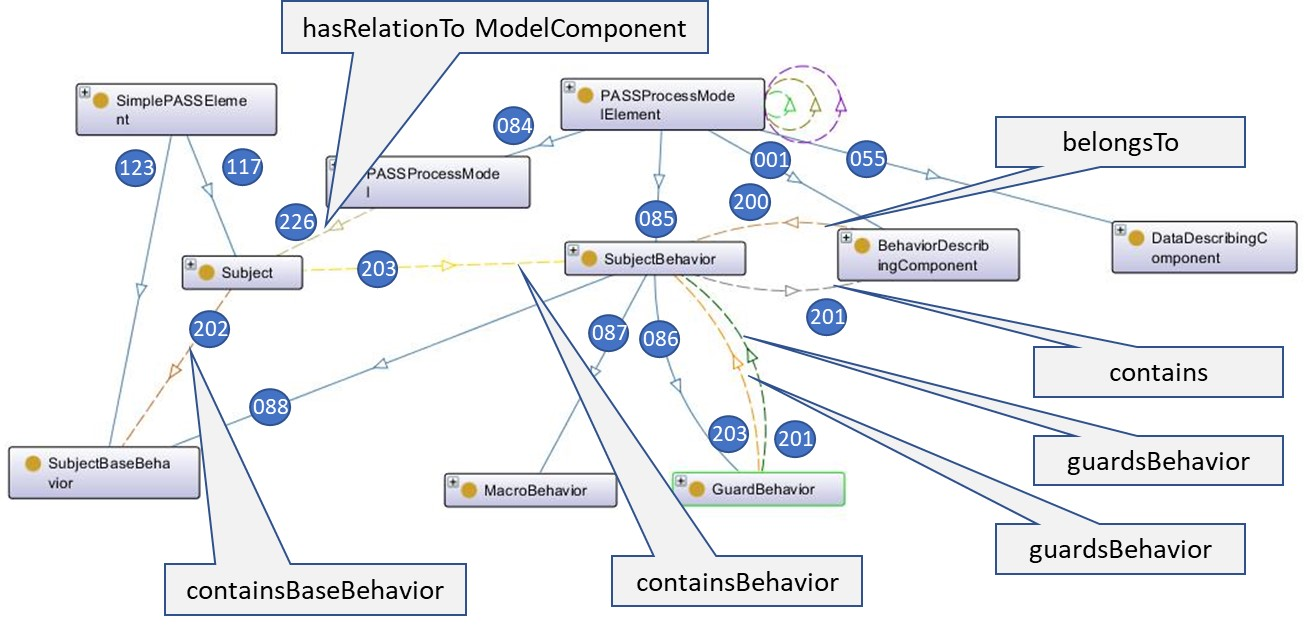
\includegraphics[width=0.9\linewidth]{Figures/Ontology/SubjectBehavior/20190104-SImple-Elements-and-Modellelement}
	\caption[Structure of Subject Behavior Specification]{Structure of Subject Behavior Specification}
	\label{fig:20190104-simple-elements-and-modellelement}
\end{figure}

\subsubsection{Behavior Describing Components}

The following figure shows the details of the class \PASSModelElement{BehaviorDescribingComponent}. This class has the important sub-classes \PASSModelElement{State}, \PASSModelElement{Transition} and \PASSModelElement{TransitionCondition} (see figure \ref{fig:20190104-behavior-describing-component}). The sub-classes of the state represent the various types of states (class relations 025, 014 and 024 in \ref{fig:20190104-behavior-describing-component}). The standard states \PASSModelElement{DoStates}, \PASSModelElement{SendState} and \PASSModelElement{ReceiveState} are sub-classes of the class \PASSModelElement{StandardPASSState} (class relations 114, 115 and 116 in \ref{fig:20190104-behavior-describing-component}). The subclass relations 104 and 020 allow that there exists a start state (class \PASSModelElement{InitialStatOfBehavior} in \ref{fig:20190104-behavior-describing-component}) and none or several end states (see subclass relation 020 in figure\ref{fig:20190104-behavior-describing-component}) The fact that there must be at least one start state and none or several end states is defined by so called axioms which are not shown in figure \ref{fig:20190104-behavior-describing-component}.

\begin{figure}[htbp]
	\centering
	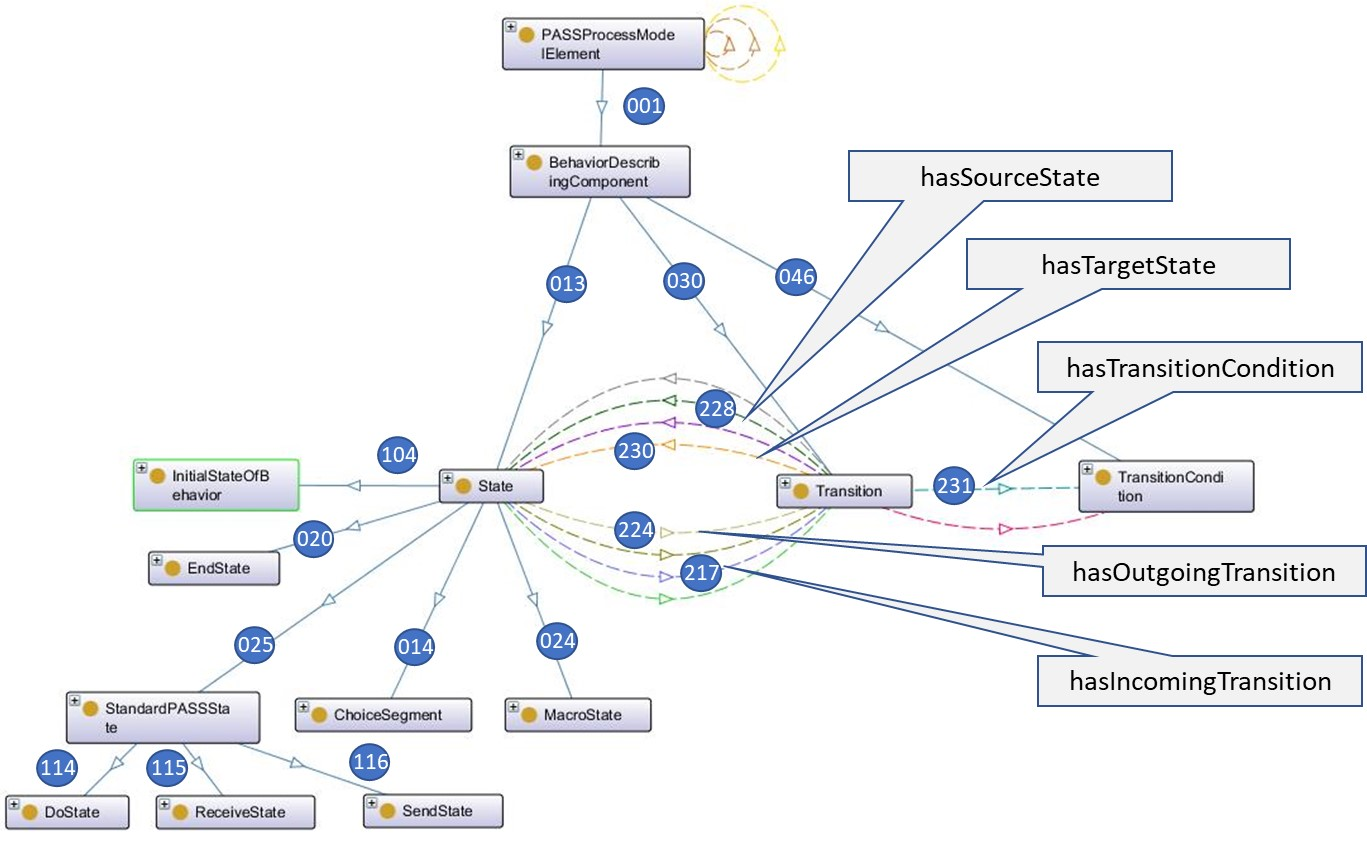
\includegraphics[width=1.0\linewidth]{Figures/Ontology/SubjectBehavior/20190104-Behavior-describing-component}
	\caption[Subject Behavior describing Component]{Subject Behavior describingComponent}
	\label{fig:20190104-behavior-describing-component}
\end{figure}

States can be starting and/or endpoints of transitions (see properties 228 and 230 in figure \ref{fig:20190104-behavior-describing-component}). This means a state may have outgoing and/or incoming transitions ( \PASSModelElementObjectPropertie{hasIncomingTransition} and \PASSModelElementObjectPropertie{hasOutgoingTransition} - see properties 224 and 217 in figure \ref{fig:20190104-behavior-describing-component}). Each transition is controlled by a Transition Condition which must be true before a behavior follows a transition from the source state to the target state.

\subsubsection{States}

As shown in figure \ref{fig:20190109-states} the class state has a subclass \PASSModelElement{StandardPASSState} (subclass relation 025) which have the subclasses \PASSModelElement{ReceiveState}, \PASSModelElement{SendState} and \PASSModelElement{DoState}(subclass relations 027, 026, 025). A state can be a start state (subclass \PASSModelElement{InitialStateOfBehavior} subclass relation 022). Besides these standard states there are macro states (subclass 024). Macro states contain a reference (subclass 029) to the corresponding macro (Property 201).

\begin{figure}[htbp]
	\centering
	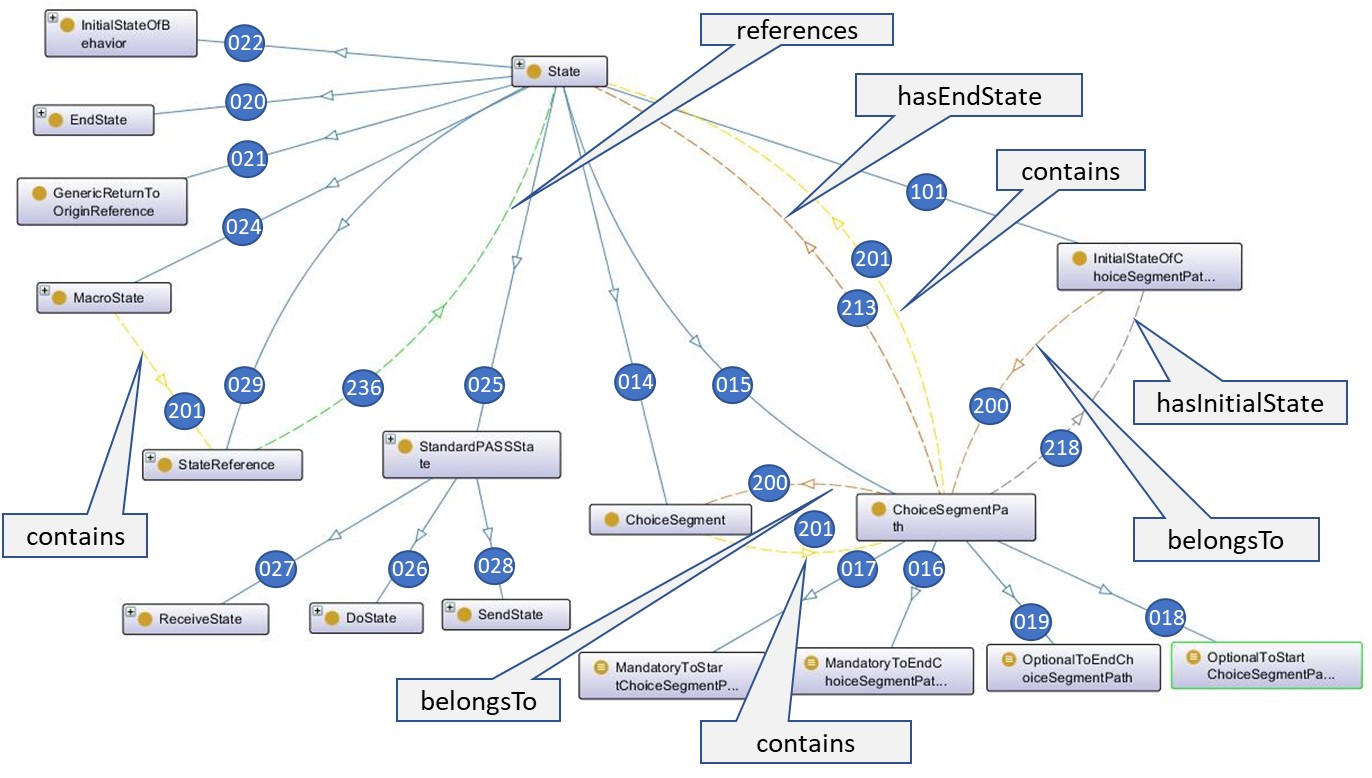
\includegraphics[width=1.0\linewidth]{Figures/Ontology/SubjectBehavior/20190109-States}
	\caption[Details of States]{Details of States}
	\label{fig:20190109-states}
\end{figure}

More complex states are choice segments (subclass relation 014). A choice segment contains choice segment paths (subclass 015 and property 200). Each choice segment path can be of one of four types. If a segment path is started then it must be finished or not, or a segment path must be started and must be finished or not (subclass relations 16, 17, 18 and 19).

\subsubsection{Transitions}

Transitions connect the source state with the target state (see figure \ref{fig:20190104-behavior-describing-component}). A transition can be executed if the transition condition is valid. This means the state of a behavior changes from the current state which is the source state to the target state. In PASS there are two basic types of transitions, \PASSModelElement{DoTransitions} and \PASSModelElement{CommunicationTranstions} (subclasses 34 and 31 in figure \ref{fig:20190105-transitions}). The class \PASSModelElement{CommunicationTransition} is divided into the sub-classes \PASSModelElement{ReceiveTransition} and \PASSModelElement{SendTransition} (sub-classes 32 and 33 in figure \ref{fig:20190105-transitions}).

Each transition has depending from its type a corresponding \PASSModelElement{Transition Condition} (property 231 in figure  \ref{fig:20190105-transitions}) which defines a condition that must be valid in order to execute/travel a transition. This can be 

\begin{figure}[htbp]
	\centering
	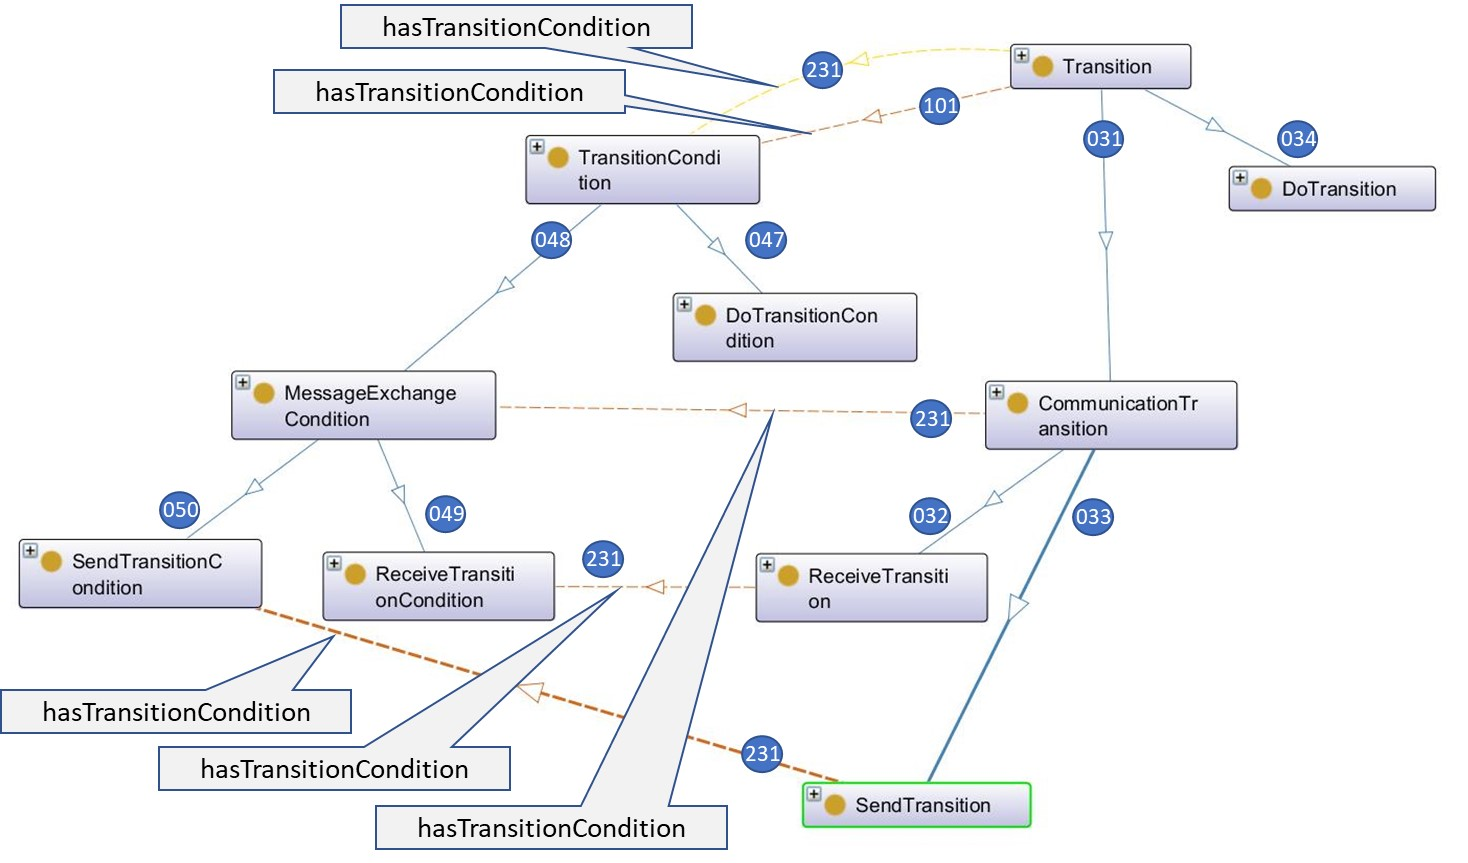
\includegraphics[width=1.0\linewidth]{Figures/Ontology/SubjectBehavior/20190105-Transitions}
	\caption[Details of transitions]{Details of transitions}
	\label{fig:20190105-transitions}
\end{figure}

Next to these main PASS transitions, the following specialized transitions exist \PASSModelElement{UserCancelTransition}s, \PASSModelElement{SendingFailedTransition}s, and \PASSModelElement{TimeTransition}s. 


\subsection{Data Describing Components}

Each subject encapsulates data (business objects). The values of these data elements can be transferred to other subjects. The following figure \ref{fig:20181218-data} shows the structure of the model components concerned with data structure description and data handling.

\begin{figure}[htbp]
	\centering
	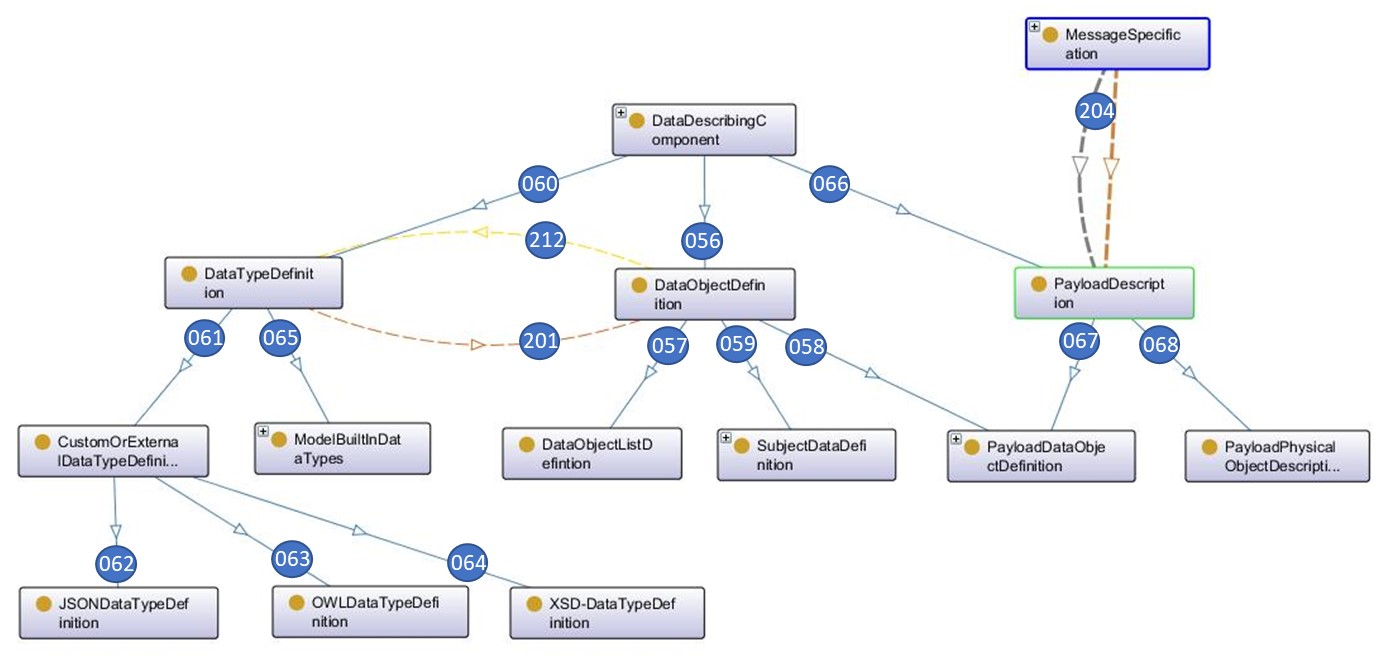
\includegraphics[width=0.9\linewidth]{Figures/Ontology/SubjectInteraction/20181218-Data}
	\caption[Data Description Component]{Data Description Component}
	\label{fig:20181218-data}
\end{figure}

Three subclasses are derived from the class \PASSModelElement{DataDescribingComponent} (in figure \ref{fig:20181218-data} are these the relations 060, 056 and 066). The subclass \PASSModelElement{PayLoadDescription} defines the data transported by messages. The relation of \PASSModelElement{PayloadDescriptions} to \PASSModelElement{MessageSpecification} is defined by the property \PASSModelElementObjectPropertie{containsPayloadDescription} (in figure \ref{fig:20181218-data} number 204).

There are two types of payloads. The class \PASSModelElement{PayloadPhysicalObjectDescription} is used if a message will be later implemented by a physical transport like a parcel in models that describe such concepts. The class \PASSModelElement{PayLoadDataObjectDefinition} is used to descripe data payloads (Subclass relations 068 and 67 in figure \ref{fig:20181218-data}). These payload objects are also a subclass of the class \PASSModelElement{DataObjectDefinition} (Subclass relation 058 in figure \ref{fig:20181218-data}).

Data objects have a certain type. Therefore class \PASSModelElement{DataObjectDefinition} has the relation \PASSModelElementObjectPropertie{hasDatatype} to class \PASSModelElement{DataTypeDefinition} (property 212 in figure\ref{fig:20181218-data}). Class \PASSModelElement{DataTypeDefinition} has two subclasses (subclass relations 061 and 065 in figure \ref{fig:20181218-data}). The subclass \PASSModelElement{ModelBuiltInDataTypes} are user defined data types whereas the class \PASSModelElement{CustomOfExternalDataTypeDefinition} is the superclass of JSON, OWL or XML based data type definitions(subclass relations 062, 63 and 064 in figure \ref{fig:20181218-data}).